Borrar todas las órdenes de la ciudad Utah que tengan artículos de la subcategoría \textbf{Tables}. \\

En este caso, lo primero que hacemos es realizar un natural join entre \textit{orders}, \textit{customer} y \textit{products}, almacenando dicho join en una relación temporal \textit{r}. Luego, seleccionamos las tuplas que sean de la ciudad \textbf{Utah} y que tengan artículos de la subcategoría \textbf{Tables}, guardando estas tuplas en otra relación temporal \textit{s}. A continuación, hacemos una proyección de los IDs de la relación \textit{s} creada anteriormente (llamamos a esto \textit{ordenes\_a\_borrar}). Finalmente, hacemos una diferencia entre \textit{orders} y el join natural derivado de \textit{orders} y \textit{ordenes\_a\_borrar}. \\

La consulta en algebra relacional se veria de la siguiente manera: \\

\begin{center}
    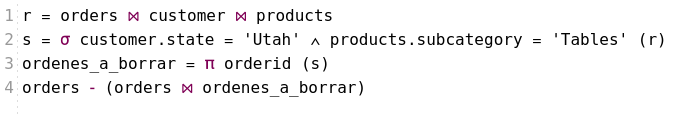
\includegraphics[width=14cm]{resources/pregunta2/3.2.1.png} \\
\end{center}

Ahora el árbol de la consulta: \\

\begin{center}
    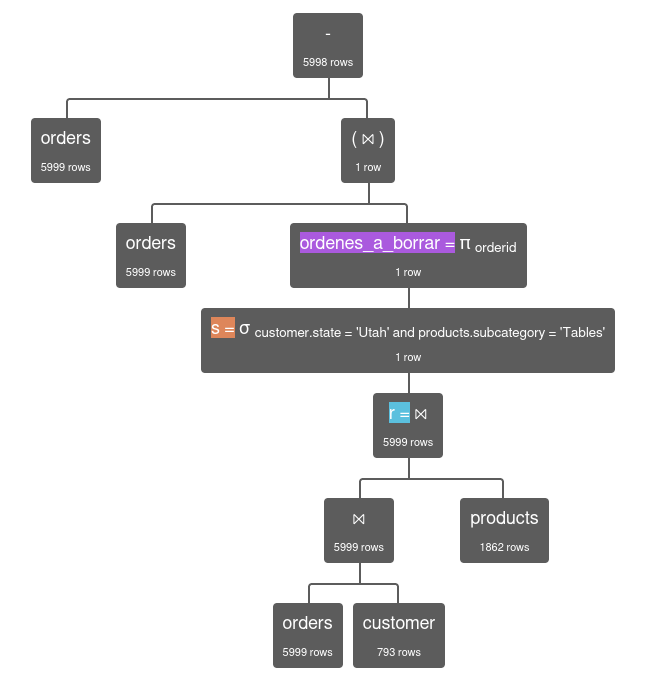
\includegraphics[width=10cm]{resources/pregunta2/3.2.2.png} \\
\end{center}

y forma de la tabla resultante: \\
\begin{center}
    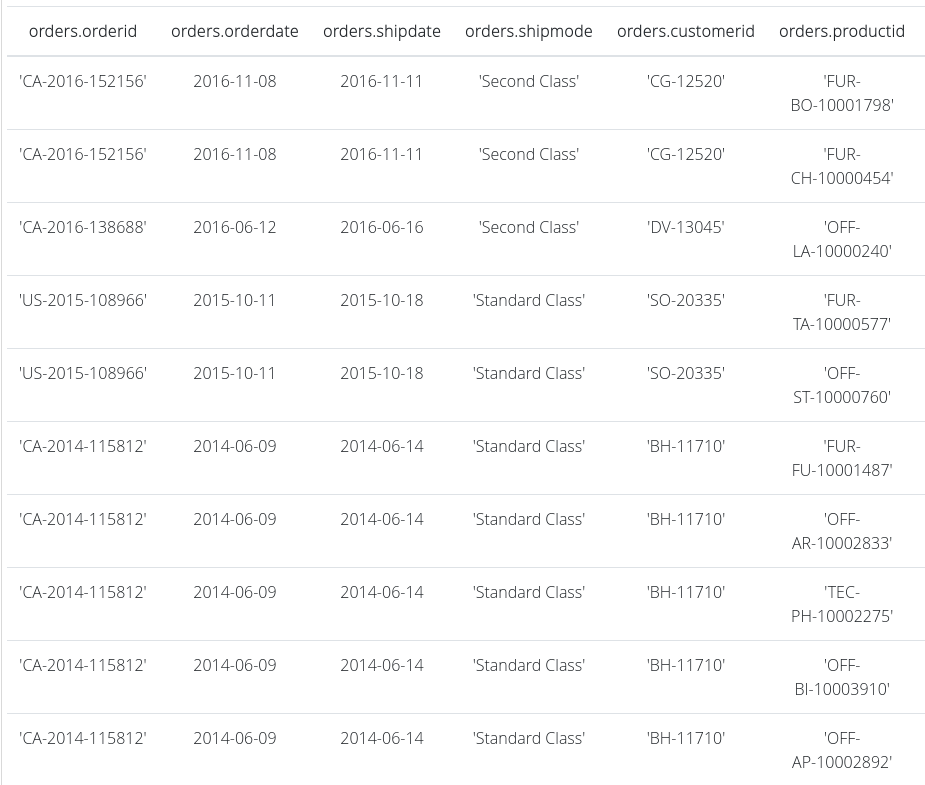
\includegraphics[width=14cm]{resources/pregunta2/3.2.3.png} \\
\end{center}